\chapter{Hoeffding Trees}
\label{chap:hoeffdingtrees} 

%This chapter describes the Hoeffding tree algorithm, chosen as the base method on which to build the MOA experimental framework of data stream classification. The reasons for choosing this algorithm are elaborated below. Most importantly, the algorithm is an ideal starting point, as it is innovative and effective at high speed data stream classification, yet it also presents opportunities for improvement.

Hoeffding trees were introduced by Domingos and Hulten in the paper ``Mining High-Speed Data Streams''~\cite{vfdt}. They refer to their implementation as {\em VFDT}, an acronym for {\bf V}ery {\bf F}ast {\bf D}ecision {\bf T}ree learner. In that paper the Hoeffding tree algorithm is the basic theoretical algorithm, while VFDT introduces several enhancements for practical implementation. In this \thesis  the term {\it Hoeffding tree} refers to any variation or refinement of the basic principle, VFDT included.

In further work Domingos and Hulten went on to show how their idea can be generalized~\cite{mineabitrarydb}, claiming that any learner based on discrete search can be made capable of processing a data stream. The key idea depends on the use of {\it Hoeffding bounds}, described in Section~\ref{sec:hoeffdingbounds}. While from this point of view VFDT may only be one instance of a more general framework, not only is it the original example and inspiration for the general framework, but because it is based on decision trees it performs very well, for reasons given shortly.

Hoeffding trees are being studied because they represent current state-of-the-art for classifying high speed data streams. The algorithm fulfills the requirements necessary for coping with data streams while remaining efficient, an achievement that was rare prior to its introduction. Previous work on scaling up decision tree learning produced systems such as {\it SLIQ}~\cite{sliq}, {\it SPRINT}~\cite{sprint} and {\it RAINFOREST}~\cite{rainforest}. These systems perform batch learning of decision trees from large data sources in limited memory by performing multiple passes over the data and using external storage. Such operations are not suitable for high speed stream processing.

Other previous systems that are more suited to data streams are those that were designed exclusively to work in a single pass, such as the incremental systems {\it ID5R}~\cite{id5r} and its successor {\it ITI}~\cite{iti}, and other earlier work on incremental learning. Systems like this were considered for data stream suitability by Domingos and Hulten, who found them to be of limited practical use. In some cases these methods require more effort to update the model incrementally than to rebuild the model from scratch. In the case of ITI, all of the previous training data must be retained in order to revisit decisions, prohibiting its use on large data sources. 

The Hoeffding tree induction algorithm induces a decision tree from a data stream incrementally, briefly inspecting each example in the stream only once, without need for storing examples after they have been used to update the tree. The only information needed in memory is the tree itself, which stores sufficient information in its leaves in order to grow, and can be employed to form predictions at any point in time between processing training examples.

Domingos and Hulten present a proof guaranteeing that a Hoeffding tree will be `very close' to a decision tree learned via batch learning. This shows that the algorithm can produce trees of the same quality as batch learned trees, despite being induced in an incremental fashion. This finding is significant because batch learned decision trees are among the best performing machine learning models.
The classic decision tree learning schemes {\em C4.5}~\cite{c4.5} and {\em CART}~\cite{cart}, two similar systems that were independently developed, are widely recognised by the research community and regarded by many as de facto standards for batch learning.

There are several reasons why decision tree learners are highly regarded. They are fairly simple, the decision tree model itself being easy to comprehend. This high level of {\it interpretability} has several advantages. The decision process induced via the learning process is transparent, so it is apparent {\it how} the model works. Questions of {\it why} the model works can lead to greater understanding of a problem, or if the model manages to be successful without truly reflecting the real world, can highlight deficiencies in the data used.

The quest for accuracy means that interpretability alone will not guarantee widespread acceptance of a machine learning model. Perhaps the main reason decision trees are popular is that they are consistently accurate on a wide variety of problems. The classic decision tree systems recursively split the multi-dimensional data into smaller and smaller regions, using greedily chosen axis-orthogonal splits. This divide-and-conquer strategy is simple yet often successful at learning diverse concepts.

Another strong feature of decision trees is their efficiency.
With $n$ examples and $m$ attributes, page 197 of~\cite{weka} shows that the average cost of basic decision tree induction is $O(mn \log n)$, ignoring complexities such as numeric attributes and subtree raising. A more detailed study of tree induction complexity can be found in~\cite{dtcomplexity}.
The cost of making a decision is $O($tree depth$)$ in the worst case, where typically the depth of a tree grows logarithmically with its size.

For the batch setting, recent studies~\cite{mlcomparison} have shown that single decision trees are no longer the best off-the-shelf method. However, they are competitive when used as base models in ensemble methods. 
For this reason, ensemble methods employing Hoeffding trees are explored later in chapters~\ref{chap:improvebackground}. %and~\ref{chap:improvecompare}. 

\section{The Hoeffding Bound for Tree Induction}
\label{sec:hoeffdingbounds}

Each internal node of a standard decision tree contains a test to divide the examples, sending examples down different paths depending on the values of particular attributes. 
The crucial decision needed to construct a decision tree is when to split a node, and with which example-discriminating test.        
If the tests used to divide examples are based on a single attribute value, as is typical in classic decision tree systems, then the set of possible tests is reduced to the number of attributes.
So the problem is refined to one of deciding which attribute, if any, is the best to split on.

There exist popular and well established criteria for selecting decision tree split tests. 
Perhaps the most common is {\it information gain}, used by C4.5.
Information gain measures the average amount of `purity' that is gained in each subset of a split. The purity of the subsets is measured using {\em entropy}, which for a distribution of class labels consisting of fractions ${p}_{1},{p}_{2},...,{p}_{n}$ summing to 1, is calculated thus:

\begin{equation} \label{eq:entropy}
\mathrm{entropy}({p}_{1},{p}_{2},...,{p}_{n}) = \sum_{i=1}^{n} -{p}_{i} \log_{2} {p}_{i}
\end{equation}

Gain in information is measured by subtracting the weighted average entropy of the subsets of a split from the entropy of the class distribution before splitting. Entropy is a concept from information theory that measures the amount of information conveyed by a message in {\em bits}. Throughout this \thesis  the splitting criterion is assumed to be information gain, but this does not rule out other methods. As pointed out by Domingos and Hulten, other similar methods such as the Gini index used by CART can be just as equally applied.

The estimated information gain resulting from a split on each attribute is the heuristic used to guide split decisions. In the batch learning setting this decision is straightforward, as the attribute with the highest information gain over all of the available and applicable training data is the one used. How to make the same (or very similar) decision in the data stream setting is the innovation contributed by Domingos and Hulten. They employ the Hoeffding bound~\cite{hoeffding}, otherwise known as an additive Chernoff bound.

The Hoeffding bound states that with probability $1 - \delta$, the true mean of a random variable of range $R$ will not differ from the estimated mean after $n$ independent observations by more than:

\begin{equation} \label{eq:hbound}
\epsilon = \sqrt{\frac{R^{2}\ln(1/\delta)}{2n}}
\end{equation}

This bound is useful because it holds true regardless of the distribution generating the values, and depends only on the range of values, number of observations and desired confidence. A disadvantage of being so general is that it is more conservative than a distribution-dependent bound.
An alternative bound has been suggested by Jin and Agrawal~\cite{nip}.
The Hoeffding bound formulation is well founded and works well empirically, so tighter bounds are not explored in this \thesisc. 

For the purposes of deciding which attribute to split on, the random variable being estimated is the difference in information gain between splitting on the best and second best attributes. For example, if the difference in gain between the best two attributes is estimated to be 0.3, and $\epsilon$ is computed to be 0.1, then the bound guarantees that the maximum possible change in difference will be 0.1. From this the smallest possible difference between them in the future must be at least 0.2, which will always represent positive separation for the best attribute.

For information gain the range of values ($R$) is the base 2 logarithm of the number of possible class labels. With $R$ and $\delta$ fixed, the only variable left to change the Hoeffding bound ($\epsilon$) is the number of observations ($n$). As $n$ increases, $\epsilon$ will decrease, in accordance with the estimated information gain getting ever closer to its true value.

A simple test allows the decision, with confidence $1 - \delta$, that an attribute has superior information gain compared to others---when the difference in observed information gain is more than $\epsilon$. This is the core principle for Hoeffding tree induction, leading to the following algorithm.

\section{The Basic Algorithm}
\label{sec:basicalgorithm}

\begin{algorithm}
\caption{Hoeffding tree induction algorithm.}
\begin{algorithmic}[1]
\STATE Let $HT$ be a tree with a single leaf (the root)
\FORALL{training examples}
\STATE Sort example into leaf $l$ using $HT$
\STATE Update sufficient statistics in $l$
\STATE Increment $n_l$, the number of examples seen at $l$
\IF{$n_l$ $mod$ $n_{min}$ $= 0$ {\bf and} examples seen at $l$ not all of same class}
\STATE Compute $\overline{G}_{l}(X_{i})$ for each attribute
\STATE Let $X_{a}$ be attribute with highest $\overline{G}_{l}$
\STATE Let $X_{b}$ be attribute with second-highest $\overline{G}_{l}$
\STATE Compute Hoeffding bound $\epsilon = \sqrt{\frac{R^{2}\ln(1/\delta)}{2n_{l}}}$
\IF{$X_{a} \ne X_{\emptyset}$ {\bf and} ($\overline{G}_{l}(X_{a}) - \overline{G}_{l}(X_{b}) > \epsilon$ {\bf or} $\epsilon < \tau$)}
\STATE Replace $l$ with an internal node that splits on $X_{a}$
\FORALL{branches of the split}
\STATE Add a new leaf with initialized sufficient statistics
\ENDFOR
\ENDIF
\ENDIF
\ENDFOR
\end{algorithmic}
\label{alg:ht}
\end{algorithm}

Algorithm~\ref{alg:ht} lists pseudo-code for inducing a Hoeffding tree from a data stream.
Line 1 initializes the tree data structure, which starts out as a single root node. Lines 2-18 form a loop that is performed for every training example.

Every example is filtered down the tree to an appropriate leaf, depending on the tests present in the decision tree built to that point (line 3). This leaf is then updated (line 4)---each leaf in the tree holds the sufficient statistics needed to make decisions about further growth. The sufficient statistics that are updated are those that make it possible to estimate the information gain of splitting on each attribute. Exactly what makes up those statistics is discussed in Section~\ref{sec:suffstats}.
Line 5 simply points out that $n_l$ is the example count at the leaf, and it too is updated. Technically $n_l$ can be computed from the sufficient statistics.

For efficiency reasons the code block from lines 6-17 is only performed periodically, every $n_{min}$ examples for a particular leaf, and only when necessary, when a mix of observed classes permits further splitting. The delayed evaluation controlled by $n_{min}$ is discussed in Section~\ref{sec:graceperiod}.

Lines 7-11 perform the test described in the previous section, using the Hoeffding bound to decide when a particular attribute has won against all of the others. $G$ is the splitting criterion function (information gain) and $\overline{G}$ is its estimated value. In line 11 the test for $X_{\emptyset}$, the null attribute, is used for pre-pruning (Section~\ref{sec:preprune}). The test involving $\tau$ is used for tie-breaking (Section~\ref{sec:tiebreak}).

If an attribute has been selected as the best choice, lines 12-15 split the node, causing the tree to grow. Preventing the tree from using too much memory is the topic of Section~\ref{sec:memmanage}.

\subsection{Split Confidence}
\label{sec:splitconf}

The $\delta$ parameter used in the Hoeffding bound is one minus the desired probability that the correct attribute is chosen at every point in the tree. Because a high likelihood of correctness is desired, with probability close to one, this parameter is generally set to a small value. For the experiments described throughout the \thesisc,  $\delta$ is set to the VFDT default of $10^{-7}$.

\begin{figure}
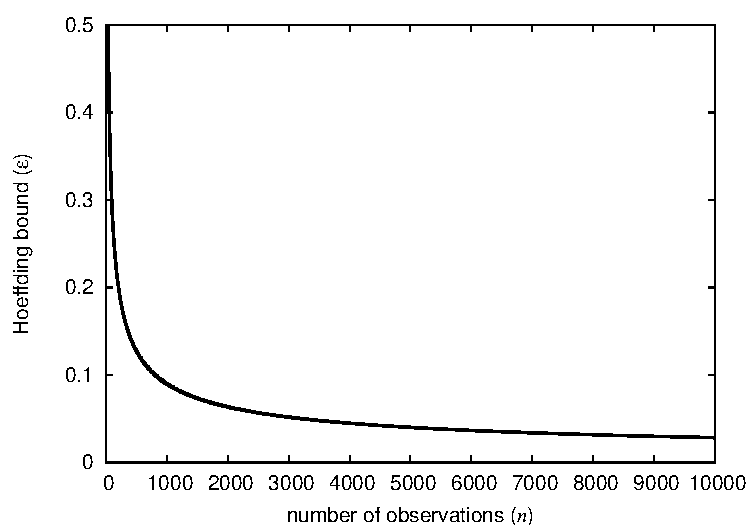
\includegraphics{figures/hoeffdingbound2class}
\caption{Hoeffding bound on a two-class problem with default parameters.}
\label{fig:hbound}
\end{figure}

Figure~\ref{fig:hbound} shows a plot of the Hoeffding bound using the default parameters for a two-class problem ($R = \mathrm{log}_{2}(2) = 1$, $\delta = 10^{-7}$). The bound rapidly drops to below 0.1 within the first one thousand examples, and after ten thousand examples is less than 0.03. This means that after ten thousand examples the calculated information gain of an attribute needs to be 0.03 greater than the second best attribute for it to be declared the winner.

\subsection{Sufficient Statistics}
\label{sec:suffstats}

The statistics in a leaf need to be sufficient to enable calculation of the information gain afforded by each possible split. Efficient storage is important---it is costly to store information in the leaves, so storing unnecessary information would result in an increase in the total memory requirements of the tree.

For attributes with discrete values, the statistics required are simply counts of the class labels that apply for each attribute value. If an attribute has $v$ unique attribute values and there are $c$ possible classes, then this information can be stored in a table with $vc$ entries. The node maintains a separate table per discrete attribute. Updating the tables simply involves incrementing the appropriate entries according to the attribute values and class of the training example.
Table~\ref{tab:leafsuffstats} on page~\pageref{tab:leafsuffstats}, used as an example when looking at prediction methods, shows what such tables can look like.

Continuous numeric attributes are more difficult to summarize. Chapter~\ref{chap:numericatts} is dedicated to this topic.

\subsection{Grace Period}
\label{sec:graceperiod}

It is computationally costly to evaluate the information gain of attributes after each and every training example. Given that a single example will have little influence on the results of the calculation, it is sensible to wait for more examples before re-evaluating. The $n_{min}$ parameter, or grace period, dictates how many examples since the last evaluation should be seen in a leaf before revisiting the decision.

This has the attractive effect of speeding up computation while not greatly harming accuracy. The majority of training time will be spent updating the sufficient statistics, a lightweight operation. Only a fraction of the time will splits be considered, a more costly procedure. The worst impact that this delay will have is a slow down of tree growth, as instead of splitting as soon as possible, a split will delayed by as much as $n_{min}-1$ examples.

For experimentation $n_{min}$ is fixed at 200, the default setting found in the original paper~\cite{vfdt}. Figure~\ref{fig:rrbfc_gp} shows the impact this setting has on the accuracy of trees induced from the {\sc rrbfc} data. From the plot in the top-left it would appear that considering split decisions after every training example does improve the accuracy of the tree, at least within the first 30 million training examples shown on this data. From an accuracy per example perspective, the non grace period tree is superior. The plot to the top-right shows more of the picture, where each tree was allowed ten hours to grow, the tree that had $n_{min}$ set to 200 was able to process almost 800 million examples and achieve significantly better accuracy within that time than the tree lacking a grace period. The plot to the bottom-left shows the total number of examples that were processed over that time---without a grace period 30 million examples in ten hours were possible, with a grace period approximately 25 times more examples were processed in the same time period. Viewing accuracy per time spent in the bottom-right plot makes the advantage of using a grace period clear.

\begin{figure}
\centering
\begin{tabular}{c@{}c}
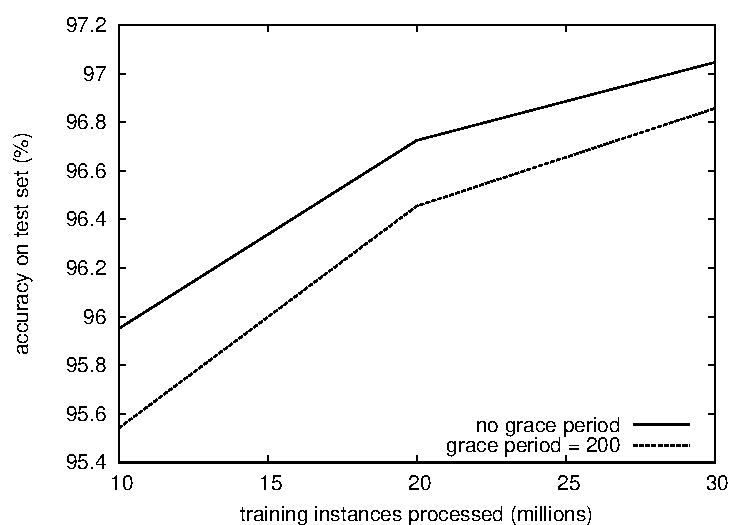
\includegraphics[width=0.5\textwidth]{figures/gp_rrbfc_acc_examples} &
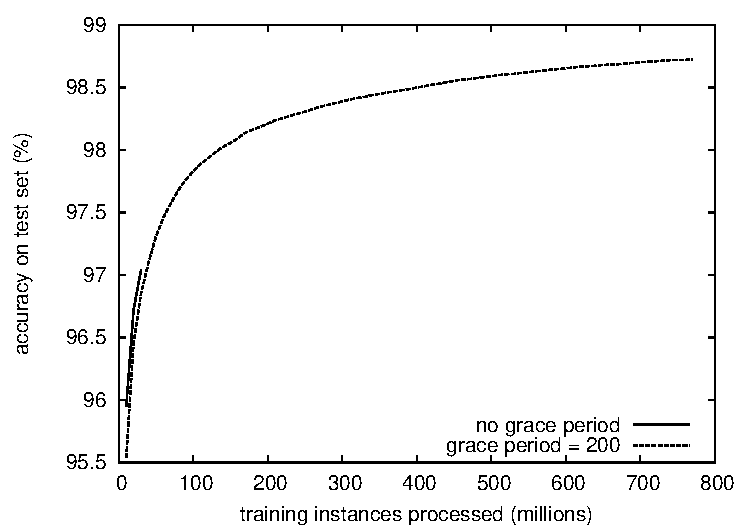
\includegraphics[width=0.5\textwidth]{figures/gp_rrbfc_acc_examples_fullrange} \\
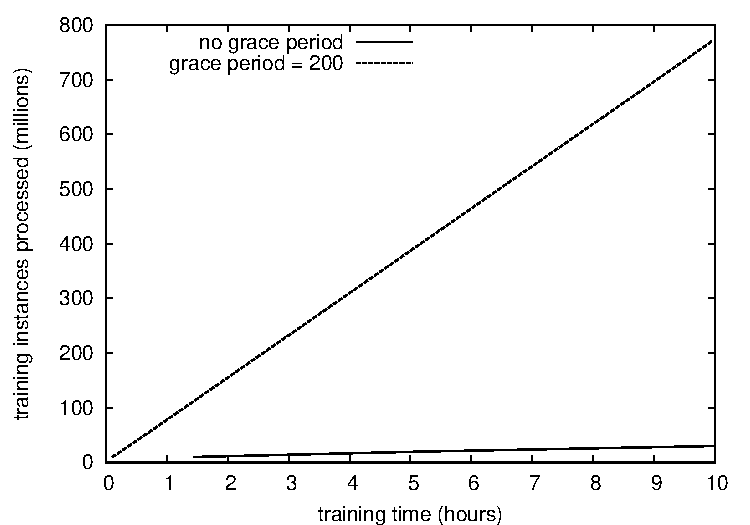
\includegraphics[width=0.5\textwidth]{figures/gp_rrbfc_time} &
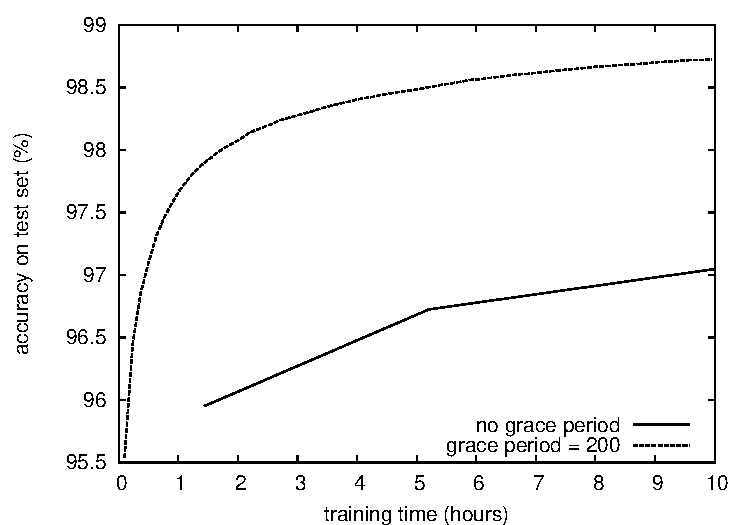
\includegraphics[width=0.5\textwidth]{figures/gp_rrbfc_acc_time} \\
\end{tabular}
\caption{Effect of grace period on the {\sc rrbfc} data with a 32MB memory limit.}
\label{fig:rrbfc_gp}
\end{figure}


\subsection{Pre-pruning}
\label{sec:preprune}

It may turn out more beneficial to not split a node at all. The Hoeffding tree algorithm detects this case by also considering the merit of no split, represented by the null attribute $X_{\emptyset}$. A node is only allowed to split when an attribute looks sufficiently better than $X_{\emptyset}$, by the same Hoeffding bound test that determines differences between other attributes.

All of the Hoeffding tree implementations used in experiments for this \thesis  had pre-pruning enabled, but revisiting some of the results without pre-pruning yielded %no noticeable differences.
no noticeable difference in size, speed or accuracy of trees.
This raises questions about the value of pre-pruning---it does not appear to be harmful and has theoretical merit, but in practice may not have an effect. This question remains open and is not further explored by this \thesisc. 

Pre-pruning in the stream setting is not a permanent decision as it is
in batch learning. Nodes are prevented from splitting until it appears
that a split will be useful, so in this sense, the memory management
strategy of disabling nodes (Section~\ref{sec:memmanage}) can also be viewed as a form of pre-pruning. Conventional knowledge about decision tree pruning is that pre-pruning can often be premature and is not as commonly used as post-pruning approaches. One reason for premature pre-pruning could be lack of sufficient data, which is not a problem in abundant data streams.

In the batch learning setting it is very easy to induce a tree that perfectly fits the training data but does not generalize to new data. This problem is typically overcome by post-pruning the tree. On non-concept drifting data streams such as those described here, it is not as critical to prevent overfitting via post-pruning as it is in the batch setting. If concept drift were present, active and adaptive post-pruning could be used to adjust for changes in concept, a topic outside the scope of this \thesisc. 

\subsection{Tie-breaking}
\label{sec:tiebreak}

A situation can arise where two or more competing attributes cannot be separated. A pathological case of this would be if there were two attributes with identical values. No matter how small the Hoeffding bound it would not be able to separate them, and tree growth would stall.

If competing attributes are equally good, and are superior to some of the other split options, then waiting too long to decide between them can do more harm than good to the accuracy of the tree. It should not make a difference which of the equal competitors is chosen. To alleviate this situation, Domingos and Hulten introduce a tie breaking parameter, $\tau$. If the Hoeffding bound is sufficiently small, that is, less than $\tau$, then the node is split on the current best attribute regardless of how close the next best option is.

The effect of this parameter can be viewed in a different way. Knowing the other variables used in the calculation of the Hoeffding bound, it is possible to compute an upper limit on the number of examples seen by a leaf before tie-breaking intervenes, forcing a split on the best observed attribute at that point. The only thing that can prevent tie-breaking is if the best option turns out to be not splitting at all, hence pre-pruning comes into effect.

$\tau$ is set to the literature default of 0.05 for the experiments. With this setting on a two-class problem, ties will be broken after 3,224 examples are observed. With $n_{min}$ being set to 200, this will actually be delayed until 3,400 examples.

Tie-breaking can have a very significant effect on the accuracy of trees produced. An example is given in Figure~\ref{fig:tiebreak_rrbfc}, where without tie-breaking the tree grows much slower, ending up around five times smaller after 700 million training examples and taking much longer to come close to the same level of accuracy as the tie-breaking variant.

\begin{figure}
\centering
\begin{tabular}{c@{}c}
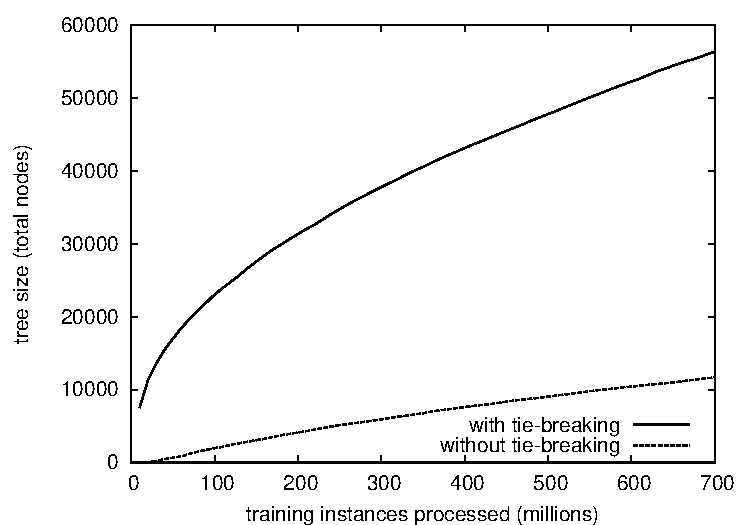
\includegraphics[width=0.5\textwidth]{figures/tiebreak_rrbfc_size} &
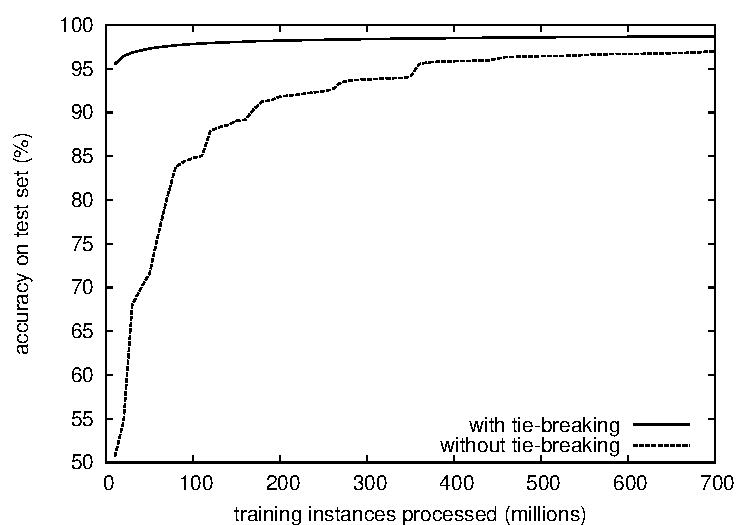
\includegraphics[width=0.5\textwidth]{figures/tiebreak_rrbfc_acc} \\
\end{tabular}
\caption{Effect of tie-breaking on the {\sc rrbfc} data with a 32MB memory limit.}
\label{fig:tiebreak_rrbfc}
\end{figure}


\subsection{Skewed Split Prevention}
\label{sec:skewedsplits}

There is another element present in the Hoeffding tree experimental implementation that is not mentioned in the pseudo-code. It is a small enhancement to split decisions that was first introduced by Gama et al.~\cite{vfdtc} and originally formulated for two-way numeric splits. In this \thesis  the concept has been generalized to apply to any split including splits with multiple branches.

The rule is that a split is only allowed if there are at least two branches where more than $p_{min}$ of the total proportion of examples are estimated to follow the branch. The $p_{min}$ threshold is an arbitrary parameter that can be adjusted, where a default value of 1\% seems to work well enough. This prevents a highly skewed split from being chosen, where less than 1\% of examples go down one path and over 99\% of examples go down another. Such a split can potentially look attractive from an information gain perspective if it increases the purity of the subsets, but from a tree growth perspective is rather spurious.

In many cases this rule has no effect on tree classification accuracy, but Figure~\ref{fig:skewedsplits_rrbfc} shows it can have a positive effect in some cases.

\begin{figure}
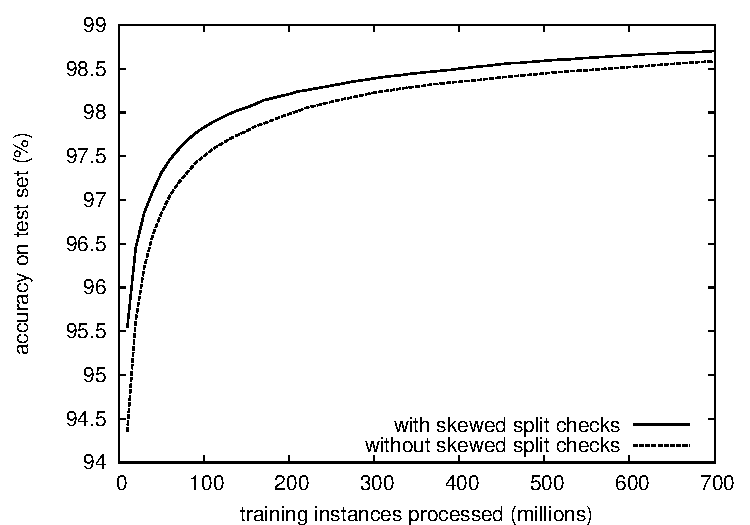
\includegraphics{figures/skewedsplits_rrbfc_acc}
\caption{Effect of preventing skewed splits on the {\sc rrbfc} data with a 32MB memory limit.}
\label{fig:skewedsplits_rrbfc}
\end{figure}

\section{Memory Management}
\label{sec:memmanage}

The basic algorithm as described will continue to split the tree as needed, without regard for the ever-increasing memory requirements. This \thesis  argues that a core requirement of data stream algorithms is the ability to limit memory usage. To limit Hoeffding tree memory size, there must be a strategy that limits the total number of nodes in the tree.
The node-limiting strategy used follows the same principles that Domingos and Hulten introduced for the VFDT system.

When looking at the memory requirements of a Hoeffding tree, the dominant cost is the storage of sufficient statistics in the leaves. Figure~\ref{fig:leaves_bytes} is an example of how closely, in unbounded memory, the number of leaves in a tree can reflect its actual memory requirements. Section~\ref{sec:fastsizeest} describes in more detail how this relationship is exploited to efficiently estimate the actual memory size of the tree based on node counts.

\begin{figure}
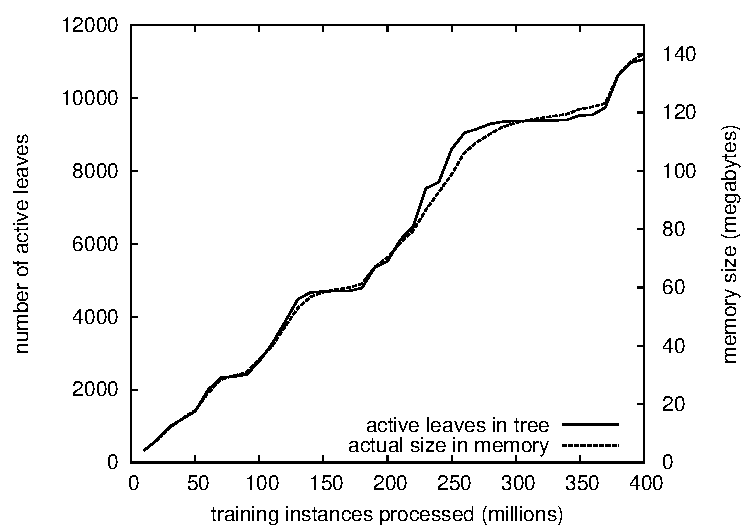
\includegraphics{figures/leaves_bytes}
\caption{The size of an unbounded tree in memory is closely related to how many active leaves it has. This growth pattern occurs when learning a Hoeffding tree on the {\sc led} data.}
\label{fig:leaves_bytes}
\end{figure}

The main idea behind the memory management strategy is that when faced with limited memory, some of the leaves can be {\em deactivated}, such that their sufficient statistics are discarded. Deciding which leaves to deactivate is based on a notion of how promising they look in terms of yielding accuracy gains for the tree.

In VFDT, the least promising nodes are defined to be the ones with the lowest values of $p_{l}e_{l}$, where $p_{l}$ is the probability that examples will reach a particular leaf $l$, and $e_{l}$ is the observed rate of error at $l$. Intuitively this makes sense, the leaves considered most promising for further splitting are those that see a high number of examples and also make a high number of mistakes. Such leaves will be the largest contributors to error in classification, so concentrating effort on splitting these nodes should see the largest reduction in error.

The implementation created for this \thesis  measures the `promise' of leaves in an equivalent and straightforward way. Every leaf in the tree is capable of returning the full count of examples it has observed for each class since creation. The promise of a node is defined as the total remaining number of examples that have been seen to fall outside the currently observed majority class. Like VFDT's $p_{l}e_{l}$ measure, this estimates the potential that a node has for misclassifying examples. If $n$ is the number of examples seen in a leaf, and $E$ is the number of mistakes made by the leaf, and $N$ is the total number of examples seen by the tree, then $p_{l}e_{l} = n/N \times E/n = E/N$. Promise is measured using $E$, which is equivalent to using $E/N$, as $N$ is constant for all leaves.

To make memory management operate without introducing excessive runtime overhead, the size is estimated approximately whenever new nodes are introduced to the tree using the method described in Section~\ref{sec:fastsizeest}. Periodically, a full and precise memory check is performed. This is done after every {\em mem-period} training examples are processed, where {\em mem-period} is a user defined constant. The periodic memory check calculates the actual memory consumption of the tree, a potentially costly process.

After checking memory usage, if there happen to be inactive nodes or if the maximum memory limit has been exceeded then a scan of the leaves is performed. The leaves are ordered from least promising to most promising, and a calculation is made based on the current sizes of the nodes to determine the maximum number of active nodes that can be supported. Once this threshold has been established, any active leaves found below the threshold are deactivated, and any inactive leaves above the threshold are reactivated. This process ensures that the tree actively and dynamically adjusts its focus on growing the most promising leaves first, while also keeping within specified memory bounds.

\begin{figure}
\centering
\framebox{
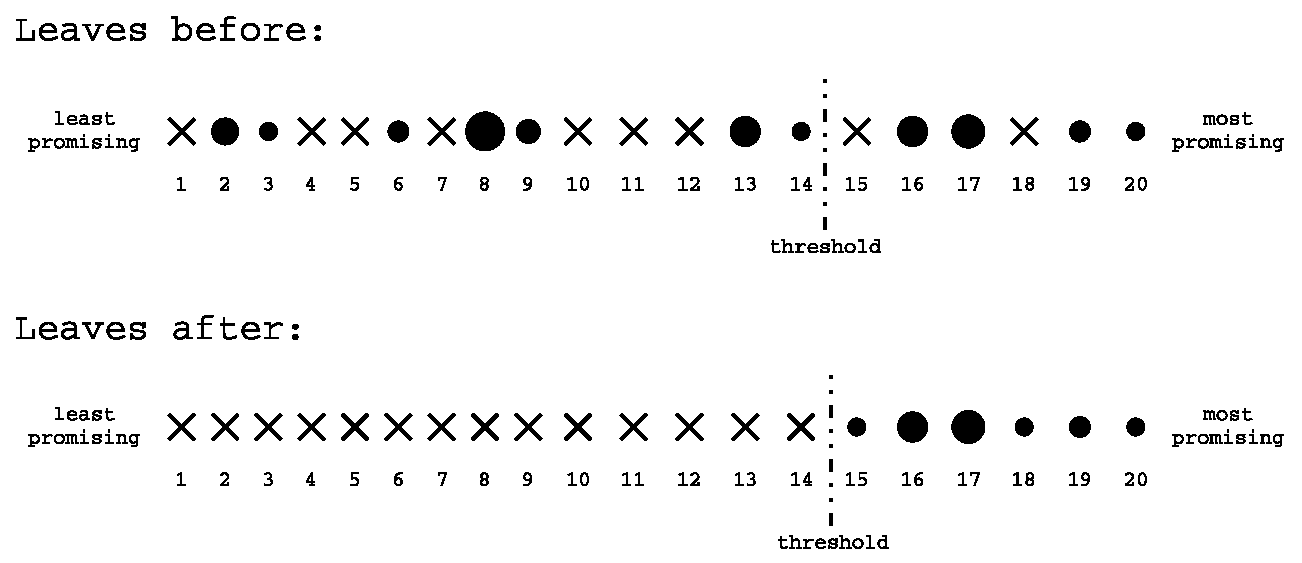
\includegraphics[width=0.95\linewidth]{figures/memmanage}
}
\caption{The memory management strategy employed after leaves of a tree have been sorted in order of {\em promise}. Dots represent {\em active} leaves which store sufficient statistics of various size, crosses represent {\em inactive} leaves which do not store sufficient statistics.}
\label{fig:memmanage}
\end{figure}

Figure~\ref{fig:memmanage} illustrates the process. The top part of the illustration shows twenty leaf nodes from a hypothetical Hoeffding tree ordered from least to most promising. The size of active nodes in memory can differ due to the method used to track numeric attributes (Chapter~\ref{chap:numericatts}) and when the sufficient statistics of poor attributes have been removed (Section~\ref{sec:pooratts}). The sizes of the dots indicate the sizes of the active nodes, and inactive nodes are represented by crosses. Based on the average size of the active nodes and the total memory allowed, the threshold is determined in this case to allow a maximum of six active nodes. The bottom row shows the outcome after memory management is complete---below the threshold, the least promising nodes have all been deactivated, and above the threshold nodes 15 and 18 have been activated to make all of the most promising ones active.

\begin{figure}
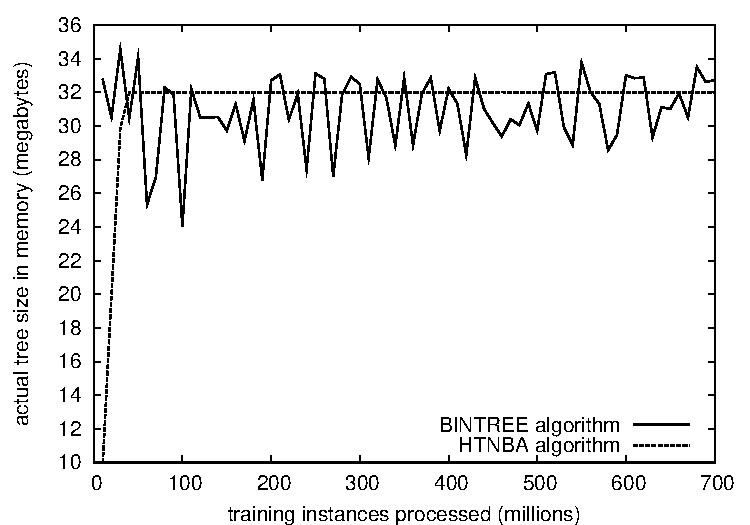
\includegraphics{figures/memslip}
\caption{How closely two algorithms manage to obey a memory limit of 32 megabytes on the {\sc led} data.}
\label{fig:memslip}
\end{figure}

For methods where the relative size between internal nodes, active leaves and inactive leaves is relatively constant this method is very effective at keeping the tree within a memory bound. For some methods where summary statistics in leaves can grow rapidly and vary substantially in size, such as the exhaustive binary tree numeric handling method ({\sc bintree}) described in Chapter~\ref{chap:numericatts}, it is less successful in maintaining a strict memory bound. In these cases, the tree's memory usage has a chance to creep beyond the limit in the period between memory checks, but will be brought back to the memory limit as soon as the next check is performed. Figure~\ref{fig:memslip} demonstrates a case of memory `creep' that occurred in the experiments---the target memory limit is 32 megabytes, and for efficiency the memory usage is only precisely measured every one hundred thousand examples, that is, {\em mem-period} = 100,000. In this case, the memory used by {\sc bintree} temporarily exceeds the memory bounds by as much as three megabytes or roughly 9\%, but all the while fluctuating close to and more often further below the desired bound. The figure compares this with the memory requirements of the {\sc htnba} variant on the same data, a much more stable method described in Chapter~\ref{chap:predstrat}. The majority of the Hoeffding tree variants tested in the experiments exhibit stable memory behaviour, so most cases look like this, where the memory plot over time hits the target precisely before completely flattening out.

While the dominant storage cost is incurred for active nodes, limiting their number will eventually cause the size of internal nodes and inactive leaves to become significant. A point will be reached where no further growth of the tree can occur without the memory limit being exceeded. Once this stage is reached, all leaves of the tree will be made inactive, and the tree will no longer be able to grow.

One element of memory usage that has not yet been accounted for is the temporary working space needed to perform operations on the tree. Implemented in a modern computer language, update and prediction operations will make several function calls, and will store values and pointers in local memory, typically using some space on a working stack. This cost, which will partly depend on implementation details, is assumed to be small and bounded such that it is insignificant compared to storage of the tree itself.

\subsection{Poor Attribute Removal}
\label{sec:pooratts}

An additional strategy for saving space was also suggested by Domingos and Hulten~\cite{vfdt}. This strategy aims to reduce the size of the sufficient statistics in each leaf. 
The idea is to discard sufficient statistics for individual attributes when it looks very unlikely that they will be selected.
When new leaves are formed, all attributes are considered as candidates for splitting. During every evaluation round that does not result in a decision to split, attributes are determined to be poor if their information gain is less than the gain of the current best attribute by more than the Hoeffding bound. According to the bound, such attributes are unlikely to be selected in that particular node of the tree, so the information tracking them in the leaf is discarded and they are ignored in split decisions from that point onward.

This strategy is not as powerful as full node deactivation, the best it can do is help to reduce the average size of leaf nodes. Theoretically this should benefit the accuracy of trees, because it will allow more leaves to remain active in limited memory. In practice the gains appear to be slight, as demonstrated in Figure~\ref{fig:pooratts}, where on {\sc rrbfc} the plot to the left shows a significant increase in the number of leaves allowed to remain active in a 32MB limit, while the plot to the right shows that this only translates to a small gain in accuracy. In this case the accuracy is measured when the tree makes predictions using standard majority class prediction. Removing poor attributes will affect the enhanced prediction methods described in Chapter~\ref{chap:predstrat}, where this is discussed further.

\begin{figure}
\centering
\begin{tabular}{c@{}c}
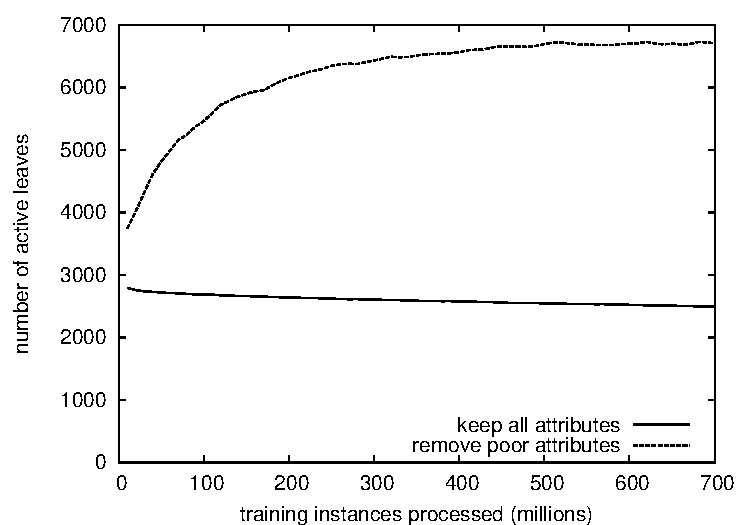
\includegraphics[width=0.5\textwidth]{figures/pooratt_active} &
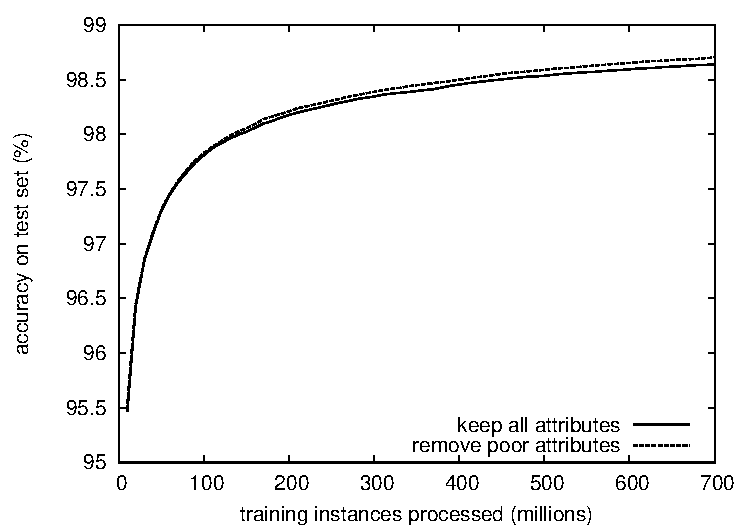
\includegraphics[width=0.5\textwidth]{figures/pooratt_acc} \\
\end{tabular}
\caption{Effect of poor attribute removal on {\sc rrbfc} data with a 32MB limit.}
\label{fig:pooratts}
\end{figure}


\section{MOA Java Implementation Details}
\label{sec:javaimpl}

%The data stream evaluation framework and all algorithms evaluated in this \thesis  were implemented in the Java programming language. The framework is named {\em MOA}, an acronym for {\bf M}assive {\bf O}nline {\bf A}nalysis, and has evolved during the course of developing this \thesisc. 

% MOA is related to {\em WEKA}\footnote{The moa and the weka are both birds native to New Zealand. The weka is a cheeky bird of similar size to a chicken. The moa was a large ostrich-like bird, an order of magnitude larger than a weka, that was hunted to extinction for its meat.}, the {\bf W}aikato {\bf E}nvironment for {\bf K}nowledge {\bf A}nalysis~\cite{weka}, which is an award-winning\footnote{Recipient of the 2005 SIGKDD Data Mining and Knowledge Discovery Service Award.} open-source workbench containing implementations of a wide range of batch machine learning methods. WEKA is also written in Java. The main benefits of Java are portability, where applications can be run on any platform with an appropriate Java virtual machine, and the strong and well-developed support libraries. Use of the language is widespread, and features such as the automatic garbage collection help to reduce programmer burden and error.

One of the key data structures used in MOA is the description of an example from a data stream. This structure borrows from WEKA, where an example is represented by an array of double precision floating point values. This provides freedom to store all necessary type of values---numeric attribute values can be stored directly, and discrete attribute values and class labels are represented by integer index values that are stored as floating point values in the array. Double precision floating point values require storage space of 64 bits, or 8 bytes. This detail can have implications for memory utilization.

A challenge in developing the system has been measuring the total sizes of objects in memory. Java deliberately hides details about how memory is allocated. This frees programmers from the burden of maintaining direct memory pointers that is otherwise typical in C programming, reducing dependence on a particular platform and eliminating a common source of error. The downside is that it makes the task of precisely measuring and limiting the memory usage of algorithms more difficult. 

Early attempts at memory measurement revolved around exploiting Java's automatic {\em serialization} mechanism. It is easy to make all objects capable of being serialized, which means that they can be written out as a flat stream of bytes to be reconstructed later. The idea was to measure the size of the serialized stream of an object, which must be related to its true size in memory. The measuring process can be performed with minimum overhead by writing the object to a dummy stream that allocates no memory but instead simply counts the total number of bytes requested during write operations. It turns out that this method, while suitable for approximate relative measurement of object size, was not precise enough to achieve the level of control needed to confidently evaluate the algorithms. Often the true size of objects would be underestimated, so that
even if the Java virtual machine was allocated a generous amount of memory it could still run into problems, strongly indicating that the serialized size estimates were inadequate.

Fortunately the release of Java 5 introduced a new mechanism allowing access to more accurate memory allocation measurements that are implementation specific. The {\em instrumentation} interface is harder to access as it requires extra work to be done by invoking the virtual machine with an {\em agent}, but once correctly set up can be queried for the size of a single object in memory. The size returned does not account for other sub-objects that are referenced, so it will not immediately return the total size of a complex data structure in memory, but this can be achieved by implementing additional code that uses {\em reflection} to traverse an entire data structure and compute the total size.

\begin{figure}
\begin{verbatim}
...
public static class ClassA implements Serializable {
   public int fieldA;
}
public static class ClassB implements Serializable {
   public int fieldA, fieldB;
}
public static class ClassC implements Serializable {
   public int fieldA, fieldB, fieldC;
}
public static class ClassD implements Serializable {
   public int fieldA, fieldB, fieldC, fieldD;
}
public static class ClassE implements Serializable {
   public int fieldA, fieldB, fieldC, fieldD, fieldE;
}
public static void main(String[] args) throws Exception {
   ClassA classAobject = new ClassA();
   ClassB classBobject = new ClassB();
   ClassC classCobject = new ClassC();
   ClassD classDobject = new ClassD();
   ClassE classEobject = new ClassE();
   ClassA[] classAarray = new ClassA[100];
   ClassB[] classBarray = new ClassB[100];
   ClassC[] classCarray = new ClassC[100];
   ClassD[] classDarray = new ClassD[100];
   ClassE[] classEarray = new ClassE[100];
   for (int i = 0; i < 100; i++) {
      classAarray[i] = new ClassA();
      classBarray[i] = new ClassB();
      classCarray[i] = new ClassC();
      classDarray[i] = new ClassD();
      classEarray[i] = new ClassE();
   }
   System.out.println("classAobject serialized size = "
                      + serializedByteSize(classAobject)
                      + " instrument size = "
                      + instrumentByteSize(classAobject));
   ...
\end{verbatim}
\caption{Java code testing two methods for measuring object sizes in memory.}
\label{fig:javacode}
\end{figure}

\begin{figure}
\begin{verbatim}
classAobject serialized size = 72 instrument size = 16
classBobject serialized size = 85 instrument size = 16
classCobject serialized size = 98 instrument size = 24
classDobject serialized size = 111 instrument size = 24
classEobject serialized size = 124 instrument size = 32
classAarray serialized size = 1124 instrument size = 2016
classBarray serialized size = 1533 instrument size = 2016
classCarray serialized size = 1942 instrument size = 2816
classDarray serialized size = 2351 instrument size = 2816
classEarray serialized size = 2760 instrument size = 3616
\end{verbatim}
\caption{Output from running the code in Figure~\ref{fig:javacode}.}
\label{fig:javaoutput}
\end{figure}

The Java code listing in Figure~\ref{fig:javacode} tests the two size measuring methods. Five simple Java classes possessing an increasing number of fields are measured, along with the size of those objects when replicated 100 times in an array. Figure~\ref{fig:javaoutput} displays the result of running the test in the same software environment as all of the experimental results reported in this \thesisc.  The results show that the serialization method has a tendency to over-estimate the size of single small objects in memory, which would be expected due to the overhead that must be required to completely describe a serialized stream. Interestingly though, serialization also has a tendency to underestimate the size of a collection of objects, where for example the size of the \verb|classA| array is estimated to be almost half of the instrumentation size. This behaviour explains the problems encountered when trying to rely on serialization measurements for experiments. The problem lies in hidden implementation details that make the serialization mechanism store information more efficiently than the virtual machine. The instrumentation measurements expose other effects that could not otherwise be predicted. There appears to be some form of {\em byte padding} effect present, where an object with a single integer field (4 bytes worth) requires the same space as one with two fields (16 bytes in both cases). The reason for this will be a technical decision on behalf of the virtual machine implementation, perhaps a byte alignment issue for the sake of efficiency. Whatever the reason, this discovery serves to highlight the value of an accurate measurement mechanism, enabling the ability to account for such nuances that could not be anticipated otherwise. 

\subsection{Fast Size Estimates}
\label{sec:fastsizeest}

For the Java implementation, the number of active and inactive nodes in a Hoeffding tree are used to estimate the total true size of the tree in memory. The node counts of a growing tree are easily maintained---whenever a new node is added an appropriate counter can be incremented, and when activating or deactivating leaves the counters are appropriately adjusted.

The size estimation procedure requires that actual measurements be performed every so often to establish and refine the parameters used for future estimation. The actual byte size in memory is measured ({\em trueSize}), along with the average byte size of individual active nodes ({\em activeSize}) and inactive nodes  ({\em inactiveSize}). From this an extra parameter is calculated:

\begin{equation} \label{eq:fastmemoverhead}
overhead = \frac{trueSize}{active \times activeSize + inactive \times inactiveSize}
\end{equation}

To increase the precision of the estimate the number of internal nodes in the tree, of similar size to inactive nodes, could also be included in the calculation. The implementation did not do this however, as the procedure described worked sufficiently well.

The estimated overhead is designed to account for the internal nodes of the tree, small inaccuracies in the node estimation procedure and any other structure associated with the tree that has otherwise not been accounted for, bringing the final estimate closer to the true value. Once these values are established, the actual byte size of the tree can be quickly estimated based solely on the number of active and inactive nodes in the tree:

\begin{equation} \label{eq:fastmemcalc}
size = (active \times activeSize + inactive \times inactiveSize) \times overhead
\end{equation}

This calculation can be quickly performed whenever the number of inactive or active leaves changes, sparing the need to do a complete rescan and measurement of the tree after every change.

\BEGINOMIT
\section{Summary}

Representing one of the current best techniques for learning to classify examples in data streams, the basic algorithm for inducing decision trees from data streams via Hoeffding bounds has been described, and various parameter settings discussed. The challenge of memory management has been described, and some issues with the actual implementation in Java examined. 
Two important aspects of Hoeffding trees have not been covered, as they are studied in the following chapters.
Creating decisions based on continuous numeric attributes is studied in Chapter~\ref{chap:numericatts}. How the tree forms predictions is studied in Chapter~\ref{chap:predstrat}. 

\ENDOMIT



